\chapter{模型}
\label{cha:model}
本章将详细介绍本文所使用的模型,首先在~\ref{sec:tf}~节介绍Transformer模型,它将作为本文实验中的单任务学习基线模型。接着在~\ref{sec:mtl_tf}~节介绍多任务Transformer的几种架构,最后在~\ref{sec:imp}~节描述了一些具体的实现细节。

在描述模型结构之前,首先阐述即将用到的几个概念:

\mypara{记号}
模型在处理输入的句子时,能够区分的最小单位即是记号。在自然语言处理中,一个记号或位置常常是一个单词,但也可以是字符,还可以是词片。将一个输入句子切分为多个记号的过程称为\emph{记号化},不同粒度模型的记号化过程对比可见表~\ref{tb:tokenize},其中中文单词级的记号化需要借助分词技术。本文中使用的是单词级模型,因此下文中提到的记号和单词所指的概念是一致的。

\mypara{词表}
用于训练模型的数据集中出现的记号集合被称为词表,该集合中元素的个数就是词表大小。词表大小是衡量数据集规模和模型参数量的一个重要指标。词表大小与模型有关,通常来说,字符级的模型词表较小,单词级的模型词表较大。

\mypara{任务}
本文中的任务是对于模型而言的,并不一定是通常意义上的任务。例如,模型需要优化多个目标函数,每个目标函数就可以看作一个任务。因此,联合训练词性标注、命名实体识别、语言模型等多个NLP任务可以被视作多任务学习;联合训练多个数据集,即使这些数据集被用于处理同一个NLP任务(如中文分词),也可以被视作多任务学习。

\mypara{隐编码}
神经网络的中间层被称为\emph{隐藏层},其前为输入层,其后为输出层。在很多用于处理NLP的神经网络(如循环网络和Transformer)中,输入句子的每一个记号在隐藏层都有对应的向量表示,我们将记号在隐藏层的向量表示称为隐编码。

\begin{table}[htb]
	\centering
	\caption{不同粒度的记号化方式}
	\begin{tabular}{cccc}
	\toprule[2pt]
	语言&粒度&输入&输出\\
	\midrule[1pt]
	\multirow{3}*{英文}&字符级&she looks lovely.&s h e l o o k s l o v e l y .\\
	&单词级&she looks lovely.&she\ \ looks\ \ lovely\ \ .\\
	&词片级&she looks lovely.&she\ \ looks\ \ love\ \ ly\ \ .\\
	\midrule[1pt]
	\multirow{2}*{中文}&字符级&她看起来很可爱。&她\ 看\ 起\ 来\ 很\ 可\ 爱\ 。\\
	&单词级&她看起来很可爱。&她\ \ 看起来\ \ 很\ \ 可爱\ \ 。\\
	\bottomrule[2pt]
	\end{tabular}
	\label{tb:tokenize}
\end{table}

接着,我们从数据的角度介绍神经网络模型处理NLP问题时的一般过程。

\begin{figure}[htb]
	\centering
	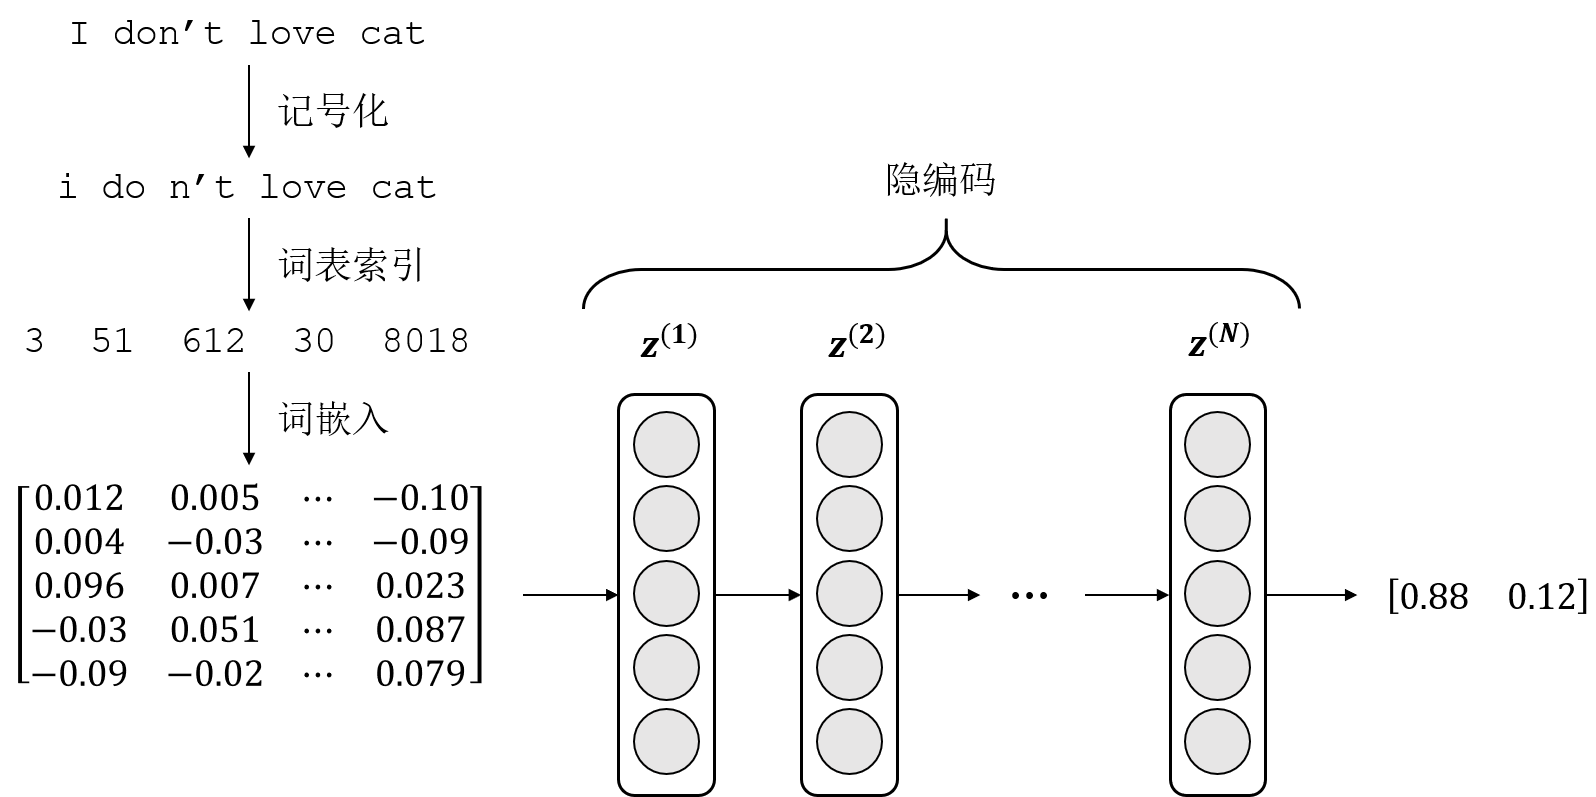
\includegraphics[scale=0.55]{nlp_pipline.png}
	\caption{神经网络处理NLP问题的一般过程}
	\label{fig:nlp_ppl}
\end{figure}

\section{Transformer}
\label{sec:tf}
Transformer是Google于2017年提出的一种完全基于\emph{自注意力}(self-attention)的全连接神经网络\cite{DBLP:conf/nips/VaswaniSPUJGKP17},摒弃了之前常用的循环计算和卷积结构,又同时具备了卷积网络的并行计算特性以及循环网络的处理长距离依赖的能力。Transformer最初被用在机器翻译中,因此包含一个\emph{编码器}和一个\emph{解码器},这里仅介绍本文用到的编码器部分\footnote{解码器的构成与编码器十分类似,只是增加了与输入端的注意力交互。}。
\begin{figure}[htb]
	\centering
	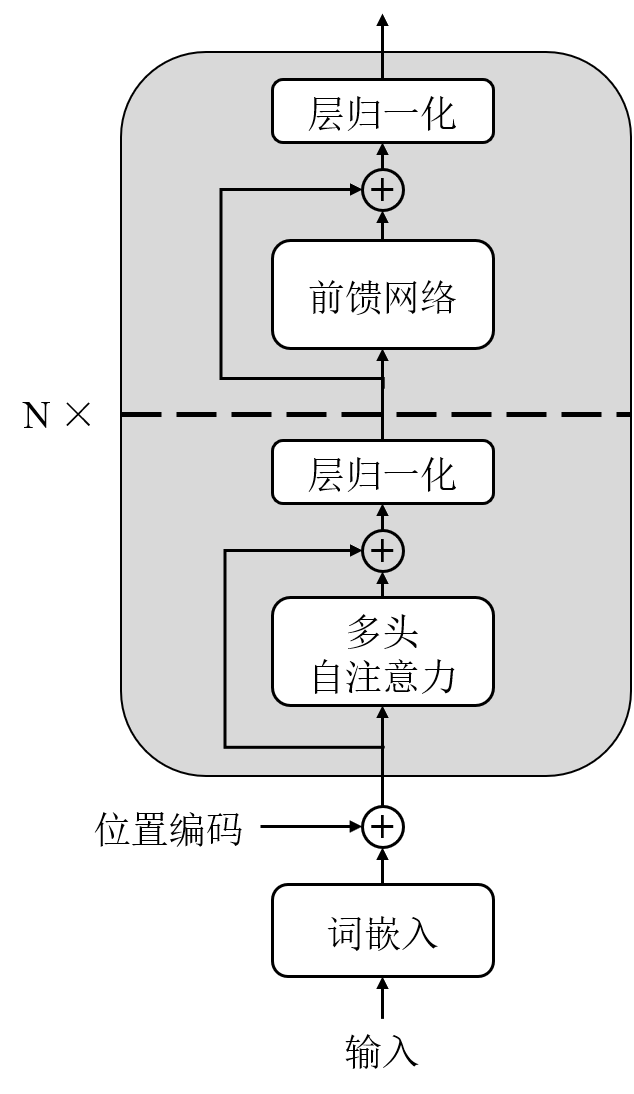
\includegraphics[scale=0.55]{tf.png}
	\caption{Transformer编码器架构}
	\label{fig:tf_encoder}
\end{figure}

作为编码器,Transformer与卷积网络、循环网络的目标一致,都是将输入的句子序列~$(x_1, x_2, ..., x_n)$~映射成一组低维稠密的向量表示~$\mathbf{z} = (\mathbf{z}_1, \mathbf{z}_2, ..., \mathbf{z}_n)$. 其中,每个位置的编码~$\mathbf{z}_i \in \mathbb{R}^{d}$. 给定~$\mathbf{z}$,解码器根据任务的不同生成不同的预测,如文本分类任务中生成文本类别~$y$,在序列标注任务中生成每个单词的标签~$(y_1, y_2, ..., y_n)$。

以分类任务为例,生成预测的过程通常使用一线性层再加一Softmax层,即:
\begin{equation}
	\hat{y} = \mathrm{softmax}(\mathbf{w}^\top \mathbf{z} + b).
\end{equation}
其中,$\mathbf{w}\in \mathbb{R}^{d\times c}$,$c$~为类别个数。

Transformer编码器的结构如图~\ref{fig:tf_encoder}~所示,图中阴影部分表示Transformer的一层,左侧的~$N$~表示层数。每一层包含两个子层:第一个子层是一个多头自注意力模块,第二个子层是一个简单的全连接前馈网络。在每个子层都有残差连接\cite{DBLP:conf/cvpr/HeZRS16}和层归一化\cite{lei2016layer}来优化训练过程。因此,每一个子层的输出为~$\mathrm{LayerNorm}(x+\mathrm{Sublayer}(x))$,其中~$\mathrm{LayerNorm}$~为层归一化,$\mathrm{Sublayer}(x)$~表示对应子层实现的函数,即多头自注意力和前馈网络。

下面先介绍第一个子层,该子层主要由多头自注意力模块构成。

\subsection{自注意力}
注意力机制就是把一\emph{查询}向量和一组\emph{键}-\emph{值}对映射为输出,这里的输入、查询(Query)、键(Key)、值(Value)、输出都为向量\footnote{为简便起见,下面的公式中不再对向量加粗表示。}。输出向量由值向量加权得到,每个值向量的权重由查询和键向量计算得出,查询和键向量的计算方式有点积、双线性等形式,Transformer使用的是一种缩放的点积形式。

自注意力是指查询、键、值都出自输入本身。假设有一个向量序列输入~$H = [h_1, \hdots, h_n]^\top \in \mathbb{R}^{n\times d}$,其中~$n$~为句子长度,$d$~为输入维度,则自注意力的计算方式为:
\begin{equation}
	\mathrm{Attention}(Q,K,V) = \mathrm{softmax}(\frac{QK^\top}{\sqrt{d_k}})V
\end{equation}
其中,$Q=HW^Q, K=HW^K, V=HW^V$\ 且\ $W^Q, W^K, W^V\in \mathbb{R}^{d\times d_k}$. 

\subsection{多头自注意力}
为了捕获更丰富的语义模式,提取句子元素之间更多的交互信息,Transformer使用了\emph{多头自注意力}(multi-head self-attention)机制:
\begin{equation}
	\begin{aligned}
	\mathrm{MultiHead}(Q,K,V)& = \mathrm{Concat}(\mathrm{head_1}, \hdots, \mathrm{head_h})W^O
	\\
	\mathrm{head_i} &= \mathrm{Attention}(HW_i^Q, HW_i^K, HW_i^V).
	\end{aligned}
\end{equation}
这里,Concat表示拼接,每个头的维度就是~$d_k$,输出矩阵~$W^O\in \mathbb{R}^{d_kh \times d}$. 在提出Transformer的论文中,作者设置~$d_k=d/h$,即令隐层维度被头的个数整除。

因此,第一个子层即是通过多头自注意力对整个输入句子进行建模。同时,这种建模方式是全局的,即句子中的每个位置都可以看到其他所有位置,因此在时间步上是全连接的。

\subsection{前馈网络}
第二个子层主要由一单隐层全连接前馈网络构成,其输入为第一个子层的输出。假设第一个子层的输出为~$x\in \mathbb{R}^{n\times d}$,则前馈网络的输出为:
\begin{equation}
	\mathrm{FFN}(x) = \max(0, xW_1+b_1)W_2+b_2.
\end{equation}
其中,$W_1 \in \mathbb{R}^{d\times d_{ff}}, W_2 \in \mathbb{R}^{d_{ff} \times d}$,$d_{ff}$~为前馈网络的隐层神经元个数。前馈网络的隐层使用的激活函数为ReLU函数,即~$\mathrm{ReLU}(\cdot)=\max(0, \cdot)$.

需要注意的是,该前馈网络在输入句子的每个位置是共享的,即对每个位置使用相同的前馈网络,因此被称为逐点前馈网络(Point-wise Feedforward Network),在计算机视觉中,这种计算方式也被称为$1\times 1$卷积。
\subsection{位置编码}
由于Transformer完全使用自注意力机制来对输入句子进行建模,无法将时序关系考虑进去,例如,对于不使用位置编码的Transformer来说,“猫坐在椅子上”和“椅子坐在猫上”两句话的表示并没有什么不同。因此需要在输入时加入额外的\emph{位置编码}(position encoding)。通常来说,加入位置编码有两种方式:一种是作为可学习的参数让模型自己学到,另一种是人为地设计对位置和维度都敏感的编码函数,例如:
\begin{equation}
	\begin{aligned}
	\mathrm{PE}_{(pos, 2i)} &= \sin(pos/10000^{2i/d})\\
	\mathrm{PE}_{(pos, 2i+1)} &= \cos(pos/10000^{2i/d})
	\end{aligned}
\end{equation}
其中,$pos$表示记号在句子中的位置,$i$表示向量维度。

最终,句中每个单词的表示由词向量与位置编码相加组成,词向量可以随机初始化,也可以使用预训练好的词向量,如word2vec,GloVe等。

至此,我们详细描述了Transformer的结构以及输入输出。容易发现,Transformer实际上就是利用注意力机制来建模句子中任意单词与其他单词之间的关系,是一种在时间步上全连接的全局建模方法。不同于传统的全连接网络,Transformer可以处理变长的句子,因为连接权重是根据输入单词来动态生成的。图~\ref{fig:tf_s}~给出了Transformer的编码过程。
\begin{figure}[htb]
	\centering
	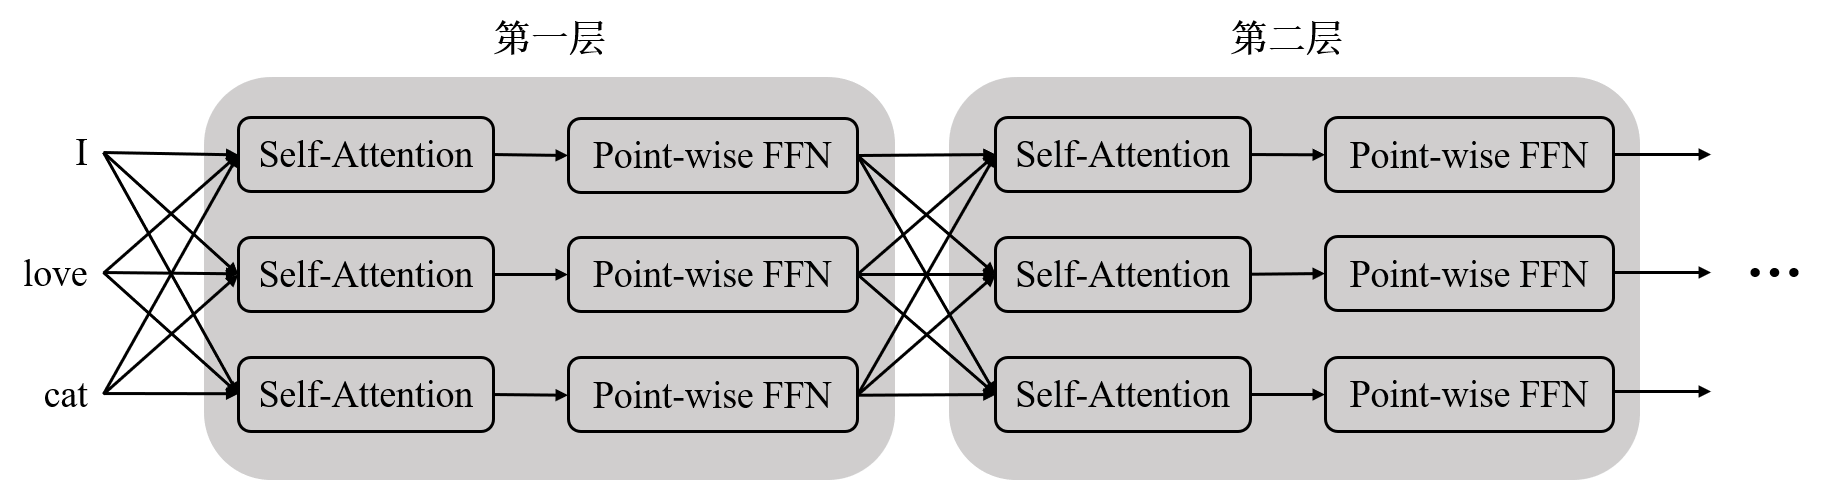
\includegraphics[scale=0.46]{tf_s.png}
	\caption{Transformer编码过程}
	\label{fig:tf_s}
\end{figure}

由于对每一位置使用了相同的前馈网络,为考虑位置之间的建模关系,可以进一步忽略掉前馈网络部分,从而可以给出一个Transformer架构的简化图~\ref{fig:tf_simp},下一节中也将基于类似的简化图来描述我们的多任务Transformer结构。
\begin{figure}[htb]
	\centering
	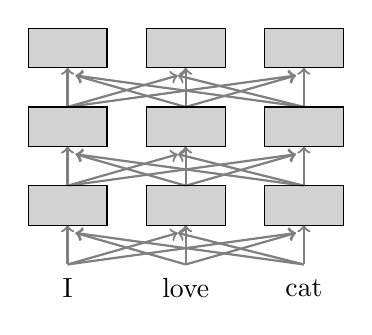
\begin{tikzpicture}
	\begin{scope}[fill opacity = .7]
	\draw [->, thick, gray ] (-1.5,0) -- (-1.5, 0.5);
	\draw [->, thick, gray ] (-1.5,0) -- (-.1, 0.4);
	\draw [->, thick, gray ] (-1.5,0) -- (1.4, 0.4);
	
	\draw [->, thick, gray ] (-1.5, 1) -- (-1.5, 1.5);
	\draw [->, thick, gray ] (-1.5, 1) -- (-.1, 1.4);
	\draw [->, thick, gray ] (-1.5, 1) -- (1.4, 1.4);
	
	\draw [->, thick, gray ] (-1.5, 2) -- (-1.5, 2.5);
	\draw [->, thick, gray ] (-1.5, 2) -- (-.1, 2.4);
	\draw [->, thick, gray ] (-1.5, 2) -- (1.4, 2.4);
	
	\draw [fill=lightgray, draw = black] (-2,1) rectangle (-1, 0.5);
	\draw [fill=lightgray, draw = black] (-2,2) rectangle (-1, 1.5);
	\draw [fill=lightgray, draw = black] (-2,3) rectangle (-1, 2.5);
	
	\draw [->, thick, gray ] (0,0) -- (0, 0.5);
	\draw [->, thick, gray ] (0,0) -- (-1.4, 0.4);
	\draw [->, thick, gray ] (0,0) -- (1.4, 0.4);
	
	\draw [->, thick, gray ] (0, 1) -- (0, 1.5);
	\draw [->, thick, gray ] (0, 1) -- (-1.4, 1.4);
	\draw [->, thick, gray ] (0, 1) -- (1.4, 1.4);
	
	\draw [->, thick, gray ] (0, 2) -- (0, 2.5);
	\draw [->, thick, gray ] (0, 2) -- (-1.4, 2.4);
	\draw [->, thick, gray ] (0, 2) -- (1.4, 2.4);
	
	\draw [fill=lightgray, draw = black] (-0.5,1) rectangle (0.5, 0.5);
	\draw [fill=lightgray, draw = black] (-0.5,2) rectangle (0.5, 1.5);
	\draw [fill=lightgray, draw = black] (-0.5,3) rectangle (0.5, 2.5);
	
	\draw [->, thick, gray ] (1.5, 0) -- (1.5, 0.5);
	\draw [->, thick, gray ] (1.5, 0) -- (-1.4, 0.4);
	\draw [->, thick, gray ] (1.5, 0) -- (-.1, 0.4);
	
	\draw [->, thick, gray ] (1.5, 1) -- (1.5, 1.5);
	\draw [->, thick, gray ] (1.5, 1) -- (-1.4, 1.4);
	\draw [->, thick, gray ] (1.5, 1) -- (-.1, 1.4);
	
	\draw [->, thick, gray ] (1.5, 2) -- (1.5, 2.5);
	\draw [->, thick, gray ] (1.5, 2) -- (-1.4, 2.4);
	\draw [->, thick, gray ] (1.5, 2) -- (-.1, 2.4);
	
	\draw [fill=lightgray, draw = black] (1,1) rectangle (2, 0.5);
	\draw [fill=lightgray, draw = black] (1,2) rectangle (2, 1.5);
	\draw [fill=lightgray, draw = black] (1,3) rectangle (2, 2.5);
	
	\end{scope}
	\node at (0, -.3) {love};
	\node at (-1.5, -.3) {I};
	\node at (1.5, -.3) {cat};
	\end{tikzpicture}
	\caption{Transformer结构的一个简化版示意图}
	\label{fig:tf_simp}
\end{figure}

\section{多任务Transformer}
\label{sec:mtl_tf}
在前文基础上,本节将展示四种基于Transformer的共享架构,其中两种为传统的硬共享模式,由于这种架构的任务特定层堆叠在共享层上面,在神经网络的顶层形成不同任务的表示,因此我们将其归纳为\emph{顶层分化};另外两种为针对Transformer的结构特点提出的共享模式,我们称之为\emph{逐层分化},即在每一层都形成任务特定表示。

对于顶层分化模式,我们给出了两种具体的实现结构:S-P结构和S-C结构。对于逐层分化模式,我们也给出了两种架构方式:L-I结构和L-E结构。

\subsection{S-P结构}
S-P意为Stack-Pooling,即\emph{堆叠-汇聚结构}。S-P结构是指在Transformer的共享层上使用信息汇聚(也称池化)的方式来得到通用句子表示。常用的池化方式一般有\emph{平均池化}(mean pooling)和\emph{最大池化}(max pooling)。以平均池化为例,假设包含~$n$~个单词的句子输入为~$x$,经过Transformer共享层之后输出的隐状态为~$z = \mathcal{F}(x) \in \mathbb{R}^{n \times d}$,对于分类任务,平均池化S-P结构的预测为
\begin{equation}
	\hat{y} = \mathrm{softmax}(\frac{1}{n}\sum_{i=1}^{n}z_i\cdot W^{(t)} + b).
	\label{eq:s-p}
\end{equation}
其中任务~$t$的分类矩阵~$W^{(t)}\in \mathbb{R}^{d\times c}$,$c$~为分类个数。在实际实现时,平均池化后先接一多层感知机(MLP)再输入softmax层常常能取得更好的效果,此时式~\ref{eq:s-p}~可写为
\begin{equation}
	\hat{y} = \mathrm{softmax}(\mathrm{MLP}(\frac{1}{n}\sum_{i=1}^{n}z_i)).
\end{equation}

图~\ref{fig:s-p}~给出了S-P结构的示意,浅灰色模块表示共享部分,深灰色模块代表整个句子的表示,$A,B,C$~代表三个不同的任务。与~\ref{sec:mtl}~节中的图示不同的是,这里的一个矩形代表一个单词的特征表示,而不是神经网络的一层。

\begin{figure}[htb]
	\centering
	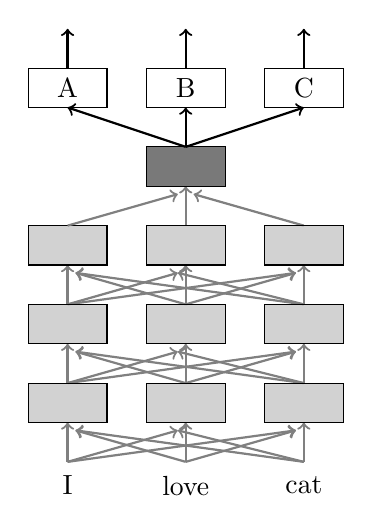
\begin{tikzpicture}
	\begin{scope}[fill opacity = .7]
	\draw [->, thick, gray ] (-1.5,0) -- (-1.5, 0.5);
	\draw [->, thick, gray ] (-1.5,0) -- (-.1, 0.4);
	\draw [->, thick, gray ] (-1.5,0) -- (1.4, 0.4);
	
	\draw [->, thick, gray ] (-1.5, 1) -- (-1.5, 1.5);
	\draw [->, thick, gray ] (-1.5, 1) -- (-.1, 1.4);
	\draw [->, thick, gray ] (-1.5, 1) -- (1.4, 1.4);
	
	\draw [->, thick, gray ] (-1.5, 2) -- (-1.5, 2.5);
	\draw [->, thick, gray ] (-1.5, 2) -- (-.1, 2.4);
	\draw [->, thick, gray ] (-1.5, 2) -- (1.4, 2.4);
	
	\draw [fill=lightgray, draw = black] (-2,1) rectangle (-1, 0.5);
	\draw [fill=lightgray, draw = black] (-2,2) rectangle (-1, 1.5);
	\draw [fill=lightgray, draw = black] (-2,3) rectangle (-1, 2.5);
	
	\draw [->, thick, gray ] (0,0) -- (0, 0.5);
	\draw [->, thick, gray ] (0,0) -- (-1.4, 0.4);
	\draw [->, thick, gray ] (0,0) -- (1.4, 0.4);
	
	\draw [->, thick, gray ] (0, 1) -- (0, 1.5);
	\draw [->, thick, gray ] (0, 1) -- (-1.4, 1.4);
	\draw [->, thick, gray ] (0, 1) -- (1.4, 1.4);
	
	\draw [->, thick, gray ] (0, 2) -- (0, 2.5);
	\draw [->, thick, gray ] (0, 2) -- (-1.4, 2.4);
	\draw [->, thick, gray ] (0, 2) -- (1.4, 2.4);
	
	\draw [->, thick, gray ] (0, 3) -- (0, 3.5);
	\draw [->, thick, gray ] (-1.5, 3) -- (-.1, 3.4);
	\draw [->, thick, gray ] (1.5, 3) -- (.1, 3.4);
	
	\draw [fill=lightgray, draw = black] (-0.5,1) rectangle (0.5, 0.5);
	\draw [fill=lightgray, draw = black] (-0.5,2) rectangle (0.5, 1.5);
	\draw [fill=lightgray, draw = black] (-0.5,3) rectangle (0.5, 2.5);
	\draw [fill=darkgray, draw = black] (-0.5,4) rectangle (0.5, 3.5);
	
	\draw [->, thick, gray ] (1.5, 0) -- (1.5, 0.5);
	\draw [->, thick, gray ] (1.5, 0) -- (-1.4, 0.4);
	\draw [->, thick, gray ] (1.5, 0) -- (-.1, 0.4);
	
	\draw [->, thick, gray ] (1.5, 1) -- (1.5, 1.5);
	\draw [->, thick, gray ] (1.5, 1) -- (-1.4, 1.4);
	\draw [->, thick, gray ] (1.5, 1) -- (-.1, 1.4);
	
	\draw [->, thick, gray ] (1.5, 2) -- (1.5, 2.5);
	\draw [->, thick, gray ] (1.5, 2) -- (-1.4, 2.4);
	\draw [->, thick, gray ] (1.5, 2) -- (-.1, 2.4);
	
	\draw [fill=lightgray, draw = black] (1,1) rectangle (2, 0.5);
	\draw [fill=lightgray, draw = black] (1,2) rectangle (2, 1.5);
	\draw [fill=lightgray, draw = black] (1,3) rectangle (2, 2.5);
	
	\draw [draw = black] (-2,5) rectangle (-1, 4.5);
	\draw [draw = black] (-.5,5) rectangle (.5, 4.5);
	\draw [draw = black] (1,5) rectangle (2, 4.5);
	
	\draw [->, thick] (0, 4) -- (0, 4.5);
	\draw [->, thick] (0, 4) -- (-1.5, 4.5);
	\draw [->, thick] (0, 4) -- (1.5, 4.5);
	
	\draw [->, thick] (0, 5) -- (0, 5.5);
	\draw [->, thick] (-1.5, 5) -- (-1.5, 5.5);
	\draw [->, thick] (1.5, 5) -- (1.5, 5.5);
	
	\end{scope}
	\node at (0, -.3) {love};
	\node at (-1.5, -.3) {I};
	\node at (1.5, -.3) {cat};
	
	\node at (-1.5, 4.75) {A};
	\node at (0, 4.75) {B};
	\node at (1.5, 4.75) {C};
	
	\end{tikzpicture}
	\caption{Stack-Pooling结构}
	\label{fig:s-p}
\end{figure}

\subsection{S-C结构}
S-C意为Stack-CLS,即\emph{堆叠-CLS结构}。S-C结构是指在Transformer的输入时添加一个\texttt{CLS}记号用来捕捉句子在每一层的表示,最后使用\texttt{CLS}的顶层表示来作为句子的通用表示。\texttt{CLS}为Classification的简写,该方法与BERT\cite{devlin2018bert}中的设置一致。

假设最顶层的\texttt{CLS}的表示为~$z_{CLS}\in \mathbb{R}^d$,则S-C结构的输出为
\begin{equation}
	\hat{y} = \mathrm{softmax}(z_{CLS}\cdot W^{(t)} + b).
	\label{eq:cls}
\end{equation}
其中任务~$t$~的分类矩阵~$W^{(t)}\in \mathbb{R}^{d\times c}$,$c$~为分类个数。图~\ref{fig:s-c}~给出了S-C结构的示意图,浅灰色为共享模块,深灰色为共享句子表示。

\begin{figure}[htb]
	\centering
	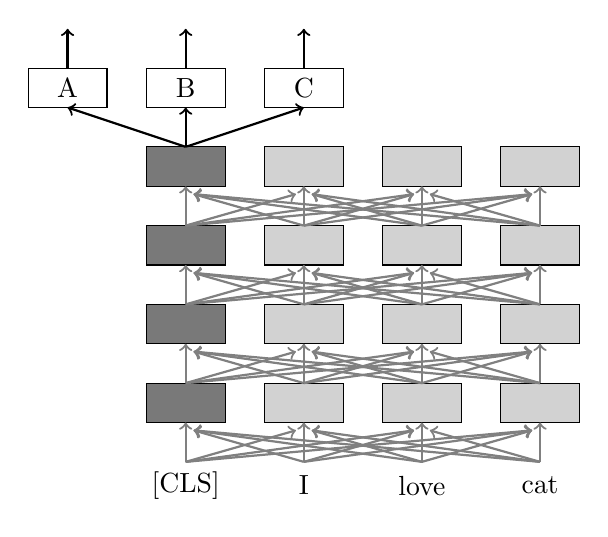
\begin{tikzpicture}
	\begin{scope}[fill opacity = .7]
	
	\draw [->, thick] (-3, 5) -- (-3, 5.5);
	\draw [->, thick] (0, 5) -- (0, 5.5);
	\draw [->, thick] (-1.5, 5) -- (-1.5, 5.5);
	
	% 中间一列
	% modules
	\draw [fill=lightgray, draw = black] (-.5, 1) rectangle (.5, .5);
	\draw [fill=lightgray, draw = black] (-.5, 2) rectangle (.5, 1.5);
	\draw [fill=lightgray, draw = black] (-.5, 3) rectangle (.5, 2.5);
	\draw [fill=lightgray, draw = black] (-.5, 4) rectangle (.5, 3.5);
	\draw [draw = black] (-.5, 5) rectangle (.5, 4.5);
	% lines
	\draw [->, thick, gray ] (0, 0) -- (0, .5);
	\draw [->, thick, gray ] (0, 0) -- (-1.4, .4);
	\draw [->, thick, gray ] (0, 0) -- (1.4, .4);
	\draw [->, thick, gray ] (0, 0) -- (2.9, .4);
	
	\draw [->, thick, gray ] (0, 1) -- (0, 1.5);
	\draw [->, thick, gray ] (0, 1) -- (-1.4, 1.4);
	\draw [->, thick, gray ] (0, 1) -- (1.4, 1.4);
	\draw [->, thick, gray ] (0, 1) -- (2.9, 1.4);
	
	\draw [->, thick, gray ] (0, 2) -- (0, 2.5);
	\draw [->, thick, gray ] (0, 2) -- (-1.4, 2.4);
	\draw [->, thick, gray ] (0, 2) -- (1.4, 2.4);
	\draw [->, thick, gray ] (0, 2) -- (2.9, 2.4);
	
	\draw [->, thick, gray ] (0, 3) -- (0, 3.5);
	\draw [->, thick, gray ] (0, 3) -- (-1.4, 3.4);
	\draw [->, thick, gray ] (0, 3) -- (1.4, 3.4);
	\draw [->, thick, gray ] (0, 3) -- (2.9, 3.4);
	
	\draw [->, thick] (-1.5, 4) -- (0, 4.5);
	
	% 左二
	% modules
	\draw [fill=darkgray, draw = black] (-2, 1) rectangle (-1, .5);
	\draw [fill=darkgray, draw = black] (-2, 2) rectangle (-1, 1.5);
	\draw [fill=darkgray, draw = black] (-2, 3) rectangle (-1, 2.5);
	\draw [fill=darkgray, draw = black] (-2, 4) rectangle (-1, 3.5);
	\draw [draw = black] (-2, 5) rectangle (-1, 4.5);
	% lines
	\draw [->, thick, gray ] (-1.5, 0) -- (-1.5, .5);
	\draw [->, thick, gray ] (-1.5, 0) -- (-.1, .4);
	\draw [->, thick, gray ] (-1.5, 0) -- (1.4, .4);
	\draw [->, thick, gray ] (-1.5, 0) -- (2.9, .4);
	
	\draw [->, thick, gray ] (-1.5, 1) -- (-1.5, 1.5);
	\draw [->, thick, gray ] (-1.5, 1) -- (-.1, 1.4);
	\draw [->, thick, gray ] (-1.5, 1) -- (1.4, 1.4);
	\draw [->, thick, gray ] (-1.5, 1) -- (2.9, 1.4);
	
	\draw [->, thick, gray ] (-1.5, 2) -- (-1.5, 2.5);
	\draw [->, thick, gray ] (-1.5, 2) -- (-.1, 2.4);
	\draw [->, thick, gray ] (-1.5, 2) -- (1.4, 2.4);
	\draw [->, thick, gray ] (-1.5, 2) -- (2.9, 2.4);
	
	\draw [->, thick, gray ] (-1.5, 3) -- (-1.5, 3.5);
	\draw [->, thick, gray ] (-1.5, 3) -- (-.1, 3.4);
	\draw [->, thick, gray ] (-1.5, 3) -- (1.4, 3.4);
	\draw [->, thick, gray ] (-1.5, 3) -- (2.9, 3.4);
	
	\draw [->, thick] (-1.5, 4) -- (-1.5, 4.5);
	
	% 最左
	% modules
	\draw [draw = black] (-3.5, 5) rectangle (-2.5, 4.5);
	% lines
	\draw [->, thick] (-1.5, 4) -- (-3, 4.5);
	
	% 右2
	% modules
	\draw [fill=lightgray, draw = black] (1, 1) rectangle (2, .5);
	\draw [fill=lightgray, draw = black] (1, 2) rectangle (2, 1.5);
	\draw [fill=lightgray, draw = black] (1, 3) rectangle (2, 2.5);
	\draw [fill=lightgray, draw = black] (1, 4) rectangle (2, 3.5);
	% lines
	\draw [->, thick, gray ] (1.5, 0) -- (1.5, .5);
	\draw [->, thick, gray ] (1.5, 0) -- (-1.4, .4);
	\draw [->, thick, gray ] (1.5, 0) -- (.1, .4);
	\draw [->, thick, gray ] (1.5, 0) -- (2.9, .4);
	
	\draw [->, thick, gray ] (1.5, 1) -- (1.5, 1.5);
	\draw [->, thick, gray ] (1.5, 1) -- (-1.4, 1.4);
	\draw [->, thick, gray ] (1.5, 1) -- (.1, 1.4);
	\draw [->, thick, gray ] (1.5, 1) -- (2.9, 1.4);
	
	\draw [->, thick, gray ] (1.5, 2) -- (1.5, 2.5);
	\draw [->, thick, gray ] (1.5, 2) -- (-1.4, 2.4);
	\draw [->, thick, gray ] (1.5, 2) -- (.1, 2.4);
	\draw [->, thick, gray ] (1.5, 2) -- (2.9, 2.4);
	
	\draw [->, thick, gray ] (1.5, 3) -- (1.5, 3.5);
	\draw [->, thick, gray ] (1.5, 3) -- (-1.4, 3.4);
	\draw [->, thick, gray ] (1.5, 3) -- (.1, 3.4);
	\draw [->, thick, gray ] (1.5, 3) -- (2.9, 3.4);
	
	
	% 最右
	% modules
	\draw [fill=lightgray, draw = black] (2.5, 1) rectangle (3.5, .5);
	\draw [fill=lightgray, draw = black] (2.5, 2) rectangle (3.5, 1.5);
	\draw [fill=lightgray, draw = black] (2.5, 3) rectangle (3.5, 2.5);
	\draw [fill=lightgray, draw = black] (2.5, 4) rectangle (3.5, 3.5);
	% lines
	\draw [->, thick, gray ] (3, 0) -- (3, .5);
	\draw [->, thick, gray ] (3, 0) -- (-1.4, .4);
	\draw [->, thick, gray ] (3, 0) -- (.1, .4);
	\draw [->, thick, gray ] (3, 0) -- (1.6, .4);
	
	\draw [->, thick, gray ] (3, 1) -- (3, 1.5);
	\draw [->, thick, gray ] (3, 1) -- (-1.4, 1.4);
	\draw [->, thick, gray ] (3, 1) -- (.1, 1.4);
	\draw [->, thick, gray ] (3, 1) -- (1.6, 1.4);
	
	\draw [->, thick, gray ] (3, 2) -- (3, 2.5);
	\draw [->, thick, gray ] (3, 2) -- (-1.4, 2.4);
	\draw [->, thick, gray ] (3, 2) -- (.1, 2.4);
	\draw [->, thick, gray ] (3, 2) -- (1.6, 2.4);
	
	\draw [->, thick, gray ] (3, 3) -- (3, 3.5);
	\draw [->, thick, gray ] (3, 3) -- (-1.4, 3.4);
	\draw [->, thick, gray ] (3, 3) -- (.1, 3.4);
	\draw [->, thick, gray ] (3, 3) -- (1.6, 3.4);
	
	\end{scope}
	
	% 输入句子
	\node at (-1.5, -.3) {[CLS]};
	\node at (0, -.3) {I};
	\node at (1.5, -.3) {love};
	\node at (3, -.3) {cat};
	
	% 任务特定层
	\node at (-3, 4.75) {A};
	\node at (-1.5, 4.75) {B};
	\node at (0, 4.75) {C};
	\end{tikzpicture}
	\caption{Stack-CLS结构}
	\label{fig:s-c}
\end{figure}

然而,在神经网络顶层形成的句子表示上进行分化得到任务特定表示的方法限制了任务特定表示对底层语义信息的使用。不同任务关注的句子信息可能在语法和语义层面都非常不同,为鼓励不同任务表示的差异化,可以在每一层都形成任务特定的表示,这就是逐层分化模式。下面介绍该模式的两种实现结构:L-I结构和L-E结构。

\subsection{L-I结构}
L-I意为Layerwise-Implicit,即\emph{层级-隐式共享结构}。首先,L-I结构将原来的\texttt{CLS}记号替换为\texttt{TASK},该记号表示任务编号,每个任务编号对应一个不同的任务向量。同时,在L-I结构中,若不同任务的类别数相同,可以不再单独设置任务特定层,不同任务通过输入不同的任务编号\texttt{TASK}来控制。

在L-I结构中,不同任务之间无法显式地交互,只能通过共享模块来隐式地交互,但不同任务在每一层都有自己的表示,因而称为层级隐式共享。L-I结构如图~\ref{fig:l-i}~所示。

\begin{figure}[htb]
	\centering
	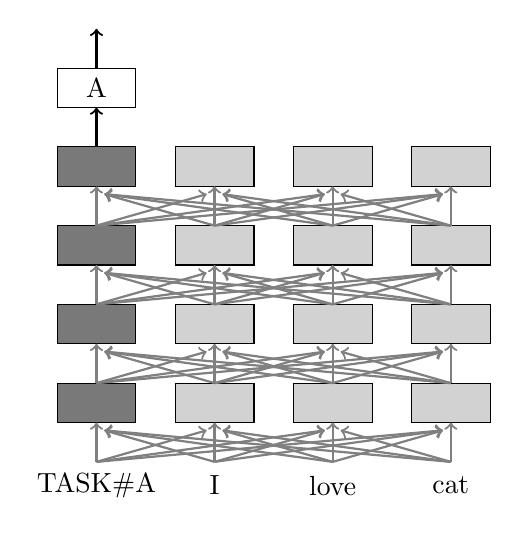
\begin{tikzpicture}
	\node at (-1.5, 4.75) {A};
	\begin{scope}[fill opacity = .7]
	
	\draw [->, thick] (-1.5, 5) -- (-1.5, 5.5);
	
	% 中间一列
	% modules
	\draw [fill=lightgray, draw = black] (-.5, 1) rectangle (.5, .5);
	\draw [fill=lightgray, draw = black] (-.5, 2) rectangle (.5, 1.5);
	\draw [fill=lightgray, draw = black] (-.5, 3) rectangle (.5, 2.5);
	\draw [fill=lightgray, draw = black] (-.5, 4) rectangle (.5, 3.5);
	% lines
	\draw [->, thick, gray ] (0, 0) -- (0, .5);
	\draw [->, thick, gray ] (0, 0) -- (-1.4, .4);
	\draw [->, thick, gray ] (0, 0) -- (1.4, .4);
	\draw [->, thick, gray ] (0, 0) -- (2.9, .4);
	
	\draw [->, thick, gray ] (0, 1) -- (0, 1.5);
	\draw [->, thick, gray ] (0, 1) -- (-1.4, 1.4);
	\draw [->, thick, gray ] (0, 1) -- (1.4, 1.4);
	\draw [->, thick, gray ] (0, 1) -- (2.9, 1.4);
	
	\draw [->, thick, gray ] (0, 2) -- (0, 2.5);
	\draw [->, thick, gray ] (0, 2) -- (-1.4, 2.4);
	\draw [->, thick, gray ] (0, 2) -- (1.4, 2.4);
	\draw [->, thick, gray ] (0, 2) -- (2.9, 2.4);
	
	\draw [->, thick, gray ] (0, 3) -- (0, 3.5);
	\draw [->, thick, gray ] (0, 3) -- (-1.4, 3.4);
	\draw [->, thick, gray ] (0, 3) -- (1.4, 3.4);
	\draw [->, thick, gray ] (0, 3) -- (2.9, 3.4);
	
	% 左二
	% modules
	\draw [fill=darkgray, draw = black] (-2, 1) rectangle (-1, .5);
	\draw [fill=darkgray, draw = black] (-2, 2) rectangle (-1, 1.5);
	\draw [fill=darkgray, draw = black] (-2, 3) rectangle (-1, 2.5);
	\draw [fill=darkgray, draw = black] (-2, 4) rectangle (-1, 3.5);
	\draw [draw = black] (-2, 5) rectangle (-1, 4.5);
	
	% lines
	\draw [->, thick, gray ] (-1.5, 0) -- (-1.5, .5);
	\draw [->, thick, gray ] (-1.5, 0) -- (-.1, .4);
	\draw [->, thick, gray ] (-1.5, 0) -- (1.4, .4);
	\draw [->, thick, gray ] (-1.5, 0) -- (2.9, .4);
	
	\draw [->, thick, gray ] (-1.5, 1) -- (-1.5, 1.5);
	\draw [->, thick, gray ] (-1.5, 1) -- (-.1, 1.4);
	\draw [->, thick, gray ] (-1.5, 1) -- (1.4, 1.4);
	\draw [->, thick, gray ] (-1.5, 1) -- (2.9, 1.4);
	
	\draw [->, thick, gray ] (-1.5, 2) -- (-1.5, 2.5);
	\draw [->, thick, gray ] (-1.5, 2) -- (-.1, 2.4);
	\draw [->, thick, gray ] (-1.5, 2) -- (1.4, 2.4);
	\draw [->, thick, gray ] (-1.5, 2) -- (2.9, 2.4);
	
	\draw [->, thick, gray ] (-1.5, 3) -- (-1.5, 3.5);
	\draw [->, thick, gray ] (-1.5, 3) -- (-.1, 3.4);
	\draw [->, thick, gray ] (-1.5, 3) -- (1.4, 3.4);
	\draw [->, thick, gray ] (-1.5, 3) -- (2.9, 3.4);
	
	\draw [->, thick] (-1.5, 4) -- (-1.5, 4.5);
	
	% 右2
	% modules
	\draw [fill=lightgray, draw = black] (1, 1) rectangle (2, .5);
	\draw [fill=lightgray, draw = black] (1, 2) rectangle (2, 1.5);
	\draw [fill=lightgray, draw = black] (1, 3) rectangle (2, 2.5);
	\draw [fill=lightgray, draw = black] (1, 4) rectangle (2, 3.5);
	% lines
	\draw [->, thick, gray ] (1.5, 0) -- (1.5, .5);
	\draw [->, thick, gray ] (1.5, 0) -- (-1.4, .4);
	\draw [->, thick, gray ] (1.5, 0) -- (.1, .4);
	\draw [->, thick, gray ] (1.5, 0) -- (2.9, .4);
	
	\draw [->, thick, gray ] (1.5, 1) -- (1.5, 1.5);
	\draw [->, thick, gray ] (1.5, 1) -- (-1.4, 1.4);
	\draw [->, thick, gray ] (1.5, 1) -- (.1, 1.4);
	\draw [->, thick, gray ] (1.5, 1) -- (2.9, 1.4);
	
	\draw [->, thick, gray ] (1.5, 2) -- (1.5, 2.5);
	\draw [->, thick, gray ] (1.5, 2) -- (-1.4, 2.4);
	\draw [->, thick, gray ] (1.5, 2) -- (.1, 2.4);
	\draw [->, thick, gray ] (1.5, 2) -- (2.9, 2.4);
	
	\draw [->, thick, gray ] (1.5, 3) -- (1.5, 3.5);
	\draw [->, thick, gray ] (1.5, 3) -- (-1.4, 3.4);
	\draw [->, thick, gray ] (1.5, 3) -- (.1, 3.4);
	\draw [->, thick, gray ] (1.5, 3) -- (2.9, 3.4);
	
	
	% 最右
	% modules
	\draw [fill=lightgray, draw = black] (2.5, 1) rectangle (3.5, .5);
	\draw [fill=lightgray, draw = black] (2.5, 2) rectangle (3.5, 1.5);
	\draw [fill=lightgray, draw = black] (2.5, 3) rectangle (3.5, 2.5);
	\draw [fill=lightgray, draw = black] (2.5, 4) rectangle (3.5, 3.5);
	% lines
	\draw [->, thick, gray ] (3, 0) -- (3, .5);
	\draw [->, thick, gray ] (3, 0) -- (-1.4, .4);
	\draw [->, thick, gray ] (3, 0) -- (.1, .4);
	\draw [->, thick, gray ] (3, 0) -- (1.6, .4);
	
	\draw [->, thick, gray ] (3, 1) -- (3, 1.5);
	\draw [->, thick, gray ] (3, 1) -- (-1.4, 1.4);
	\draw [->, thick, gray ] (3, 1) -- (.1, 1.4);
	\draw [->, thick, gray ] (3, 1) -- (1.6, 1.4);
	
	\draw [->, thick, gray ] (3, 2) -- (3, 2.5);
	\draw [->, thick, gray ] (3, 2) -- (-1.4, 2.4);
	\draw [->, thick, gray ] (3, 2) -- (.1, 2.4);
	\draw [->, thick, gray ] (3, 2) -- (1.6, 2.4);
	
	\draw [->, thick, gray ] (3, 3) -- (3, 3.5);
	\draw [->, thick, gray ] (3, 3) -- (-1.4, 3.4);
	\draw [->, thick, gray ] (3, 3) -- (.1, 3.4);
	\draw [->, thick, gray ] (3, 3) -- (1.6, 3.4);
	
	\end{scope}
	
	% 输入句子
	\node at (-1.5, -.3) {TASK\#A};
	\node at (0, -.3) {I};
	\node at (1.5, -.3) {love};
	\node at (3, -.3) {cat};
	\end{tikzpicture}
	\caption{L-I结构}
	\label{fig:l-i}
\end{figure}

L-I结构的输入为~$x=(task, x_1, x_2, ..., x_n)$,因此模型的输入层除词嵌入矩阵外还需设置一任务嵌入矩阵~$W\in \mathbb{R}^{T\times d_{t}}$,其中~$T$~为联合学习的任务个数,$d_{t}$~为任务向量的维度,可与词向量维度保持一致。在输入到Transformer后,\texttt{TASK}的计算过程与其他位置单词相同,模型应当学会根据输入的\texttt{TASK}的不同来在每一层使用注意力机制提取相应任务关注的单词信息。模型预测输出的过程与式~\ref{eq:cls}~相同。

\subsection{L-E结构}
在L-I结构基础上,我们进一步提出了L-E结构,允许任务在每一层形成自己的特定表示时能够访问其他任务的表示。L-E意为Layerwise-Explicit,即\emph{层级-显式共享结构}。L-E结构如图~\ref{fig:l-e}~所示,任务~$A$~在形成自己的表示时可以访问任务~$B$~的表示,因而这种架构是显式共享的。

\begin{figure}[htb]
	\centering
	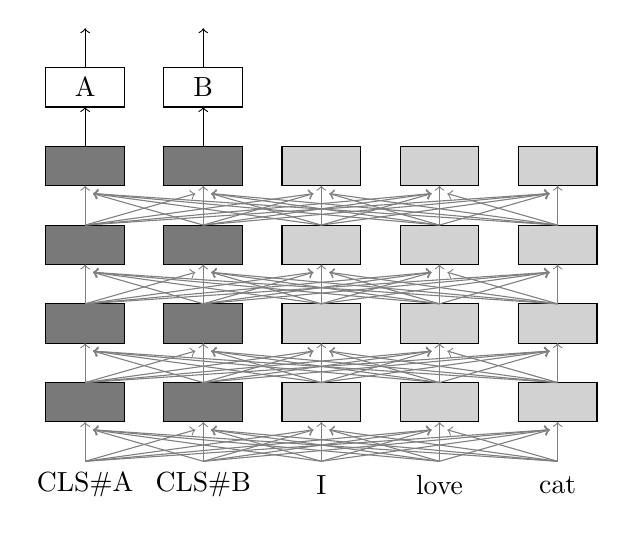
\begin{tikzpicture}
	\begin{scope}[fill opacity = .7 = .7]
	\draw [->, ] (-1.5, 5) -- (-1.5, 5.5);
	\draw [->, ] (-3, 5) -- (-3, 5.5);
	% 中间一列
	% modules
	\draw [fill=lightgray, draw = black] (-.5, 1) rectangle (.5, .5);
	\draw [fill=lightgray, draw = black] (-.5, 2) rectangle (.5, 1.5);
	\draw [fill=lightgray, draw = black] (-.5, 3) rectangle (.5, 2.5);
	\draw [fill=lightgray, draw = black] (-.5, 4) rectangle (.5, 3.5);
	% lines
	\draw [->, , gray ] (0, 0) -- (0, .5);
	\draw [->, , gray ] (0, 0) -- (-1.4, .4);
	\draw [->, , gray ] (0, 0) -- (1.4, .4);
	\draw [->, , gray ] (0, 0) -- (2.9, .4);
	\draw [->, , gray ] (0, 0) -- (-2.9, .4);
	
	\draw [->, , gray ] (0, 1) -- (0, 1.5);
	\draw [->, , gray ] (0, 1) -- (-1.4, 1.4);
	\draw [->, , gray ] (0, 1) -- (1.4, 1.4);
	\draw [->, , gray ] (0, 1) -- (2.9, 1.4);
	\draw [->, , gray ] (0, 1) -- (-2.9, 1.4);
	
	\draw [->, , gray ] (0, 2) -- (0, 2.5);
	\draw [->, , gray ] (0, 2) -- (-1.4, 2.4);
	\draw [->, , gray ] (0, 2) -- (1.4, 2.4);
	\draw [->, , gray ] (0, 2) -- (2.9, 2.4);
	\draw [->, , gray ] (0, 2) -- (-2.9, 2.4);
	
	\draw [->, , gray ] (0, 3) -- (0, 3.5);
	\draw [->, , gray ] (0, 3) -- (-1.4, 3.4);
	\draw [->, , gray ] (0, 3) -- (1.4, 3.4);
	\draw [->, , gray ] (0, 3) -- (2.9, 3.4);
	\draw [->, , gray ] (0, 3) -- (-2.9, 3.4);
	% 最左
	% modules
	\draw [fill=darkgray, draw = black] (-3.5, 1) rectangle (-2.5, .5);
	\draw [fill=darkgray, draw = black] (-3.5, 2) rectangle (-2.5, 1.5);
	\draw [fill=darkgray, draw = black] (-3.5, 3) rectangle (-2.5, 2.5);
	\draw [fill=darkgray, draw = black] (-3.5, 4) rectangle (-2.5, 3.5);
	\draw [draw = black] (-3.5, 5) rectangle (-2.5, 4.5);
	% lines
	\draw [->, , gray ] (-3, 0) -- (-3, .5);
	\draw [->, , gray ] (-3, 0) -- (-1.6, .4);
	\draw [->, , gray ] (-3, 0) -- (-.1, .4);
	\draw [->, , gray ] (-3, 0) -- (1.4, .4);
	\draw [->, , gray ] (-3, 0) -- (2.9, .4);
	
	\draw [->, , gray ] (-3, 1) -- (-3, 1.5);
	\draw [->, , gray ] (-3, 1) -- (-1.6, 1.4);
	\draw [->, , gray ] (-3, 1) -- (-.1, 1.4);
	\draw [->, , gray ] (-3, 1) -- (1.4, 1.4);
	\draw [->, , gray ] (-3, 1) -- (2.9, 1.4);
	
	\draw [->, , gray ] (-3, 2) -- (-3, 2.5);
	\draw [->, , gray ] (-3, 2) -- (-1.6, 2.4);
	\draw [->, , gray ] (-3, 2) -- (-.1, 2.4);
	\draw [->, , gray ] (-3, 2) -- (1.4, 2.4);
	\draw [->, , gray ] (-3, 2) -- (2.9, 2.4);
	
	\draw [->, , gray ] (-3, 3) -- (-3, 3.5);
	\draw [->, , gray ] (-3, 3) -- (-1.6, 3.4);
	\draw [->, , gray ] (-3, 3) -- (-.1, 3.4);
	\draw [->, , gray ] (-3, 3) -- (1.4, 3.4);
	\draw [->, , gray ] (-3, 3) -- (2.9, 3.4);
	
	\draw [->, ] (-3, 4) -- (-3, 4.5);
	
	% 左二
	% modules
	\draw [fill=darkgray, draw = black] (-2, 1) rectangle (-1, .5);
	\draw [fill=darkgray, draw = black] (-2, 2) rectangle (-1, 1.5);
	\draw [fill=darkgray, draw = black] (-2, 3) rectangle (-1, 2.5);
	\draw [fill=darkgray, draw = black] (-2, 4) rectangle (-1, 3.5);
	\draw [draw = black] (-2, 5) rectangle (-1, 4.5);
	% lines
	\draw [->, , gray ] (-1.5, 0) -- (-1.5, .5);
	\draw [->, , gray ] (-1.5, 0) -- (-.1, .4);
	\draw [->, , gray ] (-1.5, 0) -- (1.4, .4);
	\draw [->, , gray ] (-1.5, 0) -- (2.9, .4);
	\draw [->, , gray ] (-1.5, 0) -- (-2.9, .4);
	
	\draw [->, , gray ] (-1.5, 1) -- (-1.5, 1.5);
	\draw [->, , gray ] (-1.5, 1) -- (-.1, 1.4);
	\draw [->, , gray ] (-1.5, 1) -- (1.4, 1.4);
	\draw [->, , gray ] (-1.5, 1) -- (2.9, 1.4);
	\draw [->, , gray ] (-1.5, 1) -- (-2.9, 1.4);
	
	\draw [->, , gray ] (-1.5, 2) -- (-1.5, 2.5);
	\draw [->, , gray ] (-1.5, 2) -- (-.1, 2.4);
	\draw [->, , gray ] (-1.5, 2) -- (1.4, 2.4);
	\draw [->, , gray ] (-1.5, 2) -- (2.9, 2.4);
	\draw [->, , gray ] (-1.5, 2) -- (-2.9, 2.4);
	
	\draw [->, , gray ] (-1.5, 3) -- (-1.5, 3.5);
	\draw [->, , gray ] (-1.5, 3) -- (-.1, 3.4);
	\draw [->, , gray ] (-1.5, 3) -- (1.4, 3.4);
	\draw [->, , gray ] (-1.5, 3) -- (2.9, 3.4);
	\draw [->, , gray ] (-1.5, 3) -- (-2.9, 3.4);
	
	\draw [->, ] (-1.5, 4) -- (-1.5, 4.5);
	
	% 右2
	% modules
	\draw [fill=lightgray, draw = black] (1, 1) rectangle (2, .5);
	\draw [fill=lightgray, draw = black] (1, 2) rectangle (2, 1.5);
	\draw [fill=lightgray, draw = black] (1, 3) rectangle (2, 2.5);
	\draw [fill=lightgray, draw = black] (1, 4) rectangle (2, 3.5);
	% lines
	\draw [->, , gray ] (1.5, 0) -- (1.5, .5);
	\draw [->, , gray ] (1.5, 0) -- (-1.4, .4);
	\draw [->, , gray ] (1.5, 0) -- (.1, .4);
	\draw [->, , gray ] (1.5, 0) -- (2.9, .4);
	\draw [->, , gray ] (1.5, 0) -- (-2.9, .4);
	
	\draw [->, , gray ] (1.5, 1) -- (1.5, 1.5);
	\draw [->, , gray ] (1.5, 1) -- (-1.4, 1.4);
	\draw [->, , gray ] (1.5, 1) -- (.1, 1.4);
	\draw [->, , gray ] (1.5, 1) -- (2.9, 1.4);
	\draw [->, , gray ] (1.5, 1) -- (-2.9, 1.4);
	
	\draw [->, , gray ] (1.5, 2) -- (1.5, 2.5);
	\draw [->, , gray ] (1.5, 2) -- (-1.4, 2.4);
	\draw [->, , gray ] (1.5, 2) -- (.1, 2.4);
	\draw [->, , gray ] (1.5, 2) -- (2.9, 2.4);
	\draw [->, , gray ] (1.5, 2) -- (-2.9, 2.4);
	
	\draw [->, , gray ] (1.5, 3) -- (1.5, 3.5);
	\draw [->, , gray ] (1.5, 3) -- (-1.4, 3.4);
	\draw [->, , gray ] (1.5, 3) -- (.1, 3.4);
	\draw [->, , gray ] (1.5, 3) -- (2.9, 3.4);
	\draw [->, , gray ] (1.5, 3) -- (-2.9, 3.4);
	
	
	% 最右
	% modules
	\draw [fill=lightgray, draw = black] (2.5, 1) rectangle (3.5, .5);
	\draw [fill=lightgray, draw = black] (2.5, 2) rectangle (3.5, 1.5);
	\draw [fill=lightgray, draw = black] (2.5, 3) rectangle (3.5, 2.5);
	\draw [fill=lightgray, draw = black] (2.5, 4) rectangle (3.5, 3.5);
	% lines
	\draw [->, , gray ] (3, 0) -- (3, .5);
	\draw [->, , gray ] (3, 0) -- (-1.4, .4);
	\draw [->, , gray ] (3, 0) -- (.1, .4);
	\draw [->, , gray ] (3, 0) -- (1.6, .4);
	\draw [->, , gray ] (3, 0) -- (-2.9, .4);
	
	\draw [->, , gray ] (3, 1) -- (3, 1.5);
	\draw [->, , gray ] (3, 1) -- (-1.4, 1.4);
	\draw [->, , gray ] (3, 1) -- (.1, 1.4);
	\draw [->, , gray ] (3, 1) -- (1.6, 1.4);
	\draw [->, , gray ] (3, 1) -- (-2.9, 1.4);
	
	\draw [->, , gray ] (3, 2) -- (3, 2.5);
	\draw [->, , gray ] (3, 2) -- (-1.4, 2.4);
	\draw [->, , gray ] (3, 2) -- (.1, 2.4);
	\draw [->, , gray ] (3, 2) -- (1.6, 2.4);
	\draw [->, , gray ] (3, 2) -- (-2.9, 2.4);
	
	\draw [->, , gray ] (3, 3) -- (3, 3.5);
	\draw [->, , gray ] (3, 3) -- (-1.4, 3.4);
	\draw [->, , gray ] (3, 3) -- (.1, 3.4);
	\draw [->, , gray ] (3, 3) -- (1.6, 3.4);
	\draw [->, , gray] (3, 3) -- (-2.9, 3.4);
	
	\end{scope}
	
	% 输入句子
	\node at (-3, -.3) {CLS\#A};
	\node at (-1.5, -.3) {CLS\#B};
	\node at (0, -.3) {I};
	\node at (1.5, -.3) {love};
	\node at (3, -.3) {cat};
	
	\node at (-3, 4.75) {A};
	\node at (-1.5, 4.75) {B};
	\end{tikzpicture}
	\caption{L-E结构}
	\label{fig:l-e}
\end{figure}

在L-E结构输入时,为每一个任务并列地设置一个不同的\texttt{CLS}记号,因此可以看作是S-C结构的横向扩展,但L-E结构的任务特定模块被堆叠在该任务的\texttt{CLS}相对应的那一列。L-E结构允许任务在形成自己每一层的句子表示时窃听其他任务是如何抽象句子特征的。

\subsection{模型对比}
从共享模式上看,S-P结构和S-C结构都属于硬共享模式,二者结构的低层都为任务共享层。二者的区别在于S-P结构使用汇聚的方式得到句子表示,而S-C结构利用\texttt{CLS}的顶层表示作为其句子表示。L-I结构和L-E结构允许模型在每一层都形成自己的任务特定的句子表示,增大了共享的灵活性。但L-I结构在抽取自己的句子特征时无法访问其他任务抽取的特征,因此是隐式共享的;而L-E结构允许同时形成多个任务的句子表示,从而使得每个任务在抽取自己需要的特征时可以窃听其他任务的特征,因此是显式共享的。

在形式上,L-I结构和L-E结构与软共享模式类似,都允许某个任务窃听其他任务的特征。然而,L-I结构和L-E结构与之前的很多软共享方法\cite{DBLP:conf/cvpr/MisraSGH16}\cite{1705.08142}的不同之处在于,L-I结构和L-E结构可以根据输入样本的不同动态地决定与其他任务的共享程度。

\section{实现细节}
\label{sec:imp}

\subsection{训练过程}
为了避免可能出现的个别任务长时间不被选中的情况,本文采取的训练方式与一般的做法\footnote{更一般的训练方法可见文献\cite{Caruana1997}。}稍有不同。下面的算法~\ref{alg:train}~给出了具体的训练算法。

\begin{algorithm}
	\caption{多任务联合训练过程}
	\label{alg:train}
	\begin{algorithmic}[1]
		\Require $M$~个任务的数据集~$\mathcal{D}_m, 1\le m \le M$;每个任务的批量大小~$K_m, 1\le m \le M$;最大迭代次数~$T$;学习率~$\alpha$.
		\Ensure 模型参数~$\theta$.
		\Function {TrainModel}{$\mathcal{D}_m$, $K_m$, $T$, $\alpha$}
		\State 初始化模型参数$\theta_0$
		\State 初始化任务列表$L$
		\For{$t=1 \cdots T$}
			\For{$m=1 \cdots M$}
				\State 将~$\mathcal{D}_m$~划分为~$c=N_m/K_m$~个小批量集合:
				$\mathcal{B}_m = \{ \mathcal{I}_{m,1},\cdots, \mathcal{I}_{m,c} \}$
			\EndFor
			\State $i = 1$
			\While {$|L|>0$}
			\State 打乱任务列表$L$顺序
			\For {\textbf{each} $m \in L$}
			\If {$\mathcal{I}_{m,i}$存在}
			\State 计算小批量样本$\mathcal{I}_{m,i}$上的损失$\mathcal{L}$
			\State 更新参数:$\theta_t = \theta_{t-1}-\alpha \cdot \nabla_\theta \mathcal{L}(\theta) $
			\Else 
			\State 将$m$从任务列表$L$中删除
			\EndIf
			\EndFor
			\State $i = i + 1$
			\EndWhile

		\EndFor
		\State \Return $\theta_T$
		\EndFunction
	\end{algorithmic}
\end{algorithm}

在多任务联合训练时,也存在一部分较为复杂的训练策略。例如,除了通过均匀采样的方式挑选任务外,还可以按数据集比例为不同任务分配被选中的概率\cite{sanh2018hierarchical};也可以预先定义任务采样策略\cite{DBLP:journals/tacl/KiperwasserB18};还可以采用不确定性来为不同任务的损失函数分配权重\cite{DBLP:conf/cvpr/KendallGC18}。

\subsection{超参数设定}
实验中使用的均为4层Transformer,模型维度为300,包含6个头,每个头为50维,前馈网络隐层维度为512维。Transformer中的位置编码作为模型参数自动学习。使用Adam算法\cite{kingma2015adam}进行参数学习,初始学习率为5e-4,最多训练30个轮次。我们使用的小批量(mini-batch)大小为50. 

实验中采用的词向量为在840B词汇量的Common Crawl预料集上预训练的300维GloVe\cite{DBLP:conf/emnlp/PenningtonSM14}。为避免学习算法对GloVe进行过多的修改,我们为词嵌入层设置了更小的学习率:5e-5.

对于S-P结构,实现时在输出预测前叠加了一层多层感知机(MLP)以增强其效果,其余结构无此设置。前文提到的神经网络均基于fastNLP\footnote{\url{https://github.com/fastnlp/fastNLP}}和PyTorch实现,所有实验可在一张NVIDIA TITAN Xp上进行。